

nestor (Network inference from Species counTs with missingactORs) is an R package for the inference of species interaction networks from their observed abundances, while accounting for possible unobserved missing actors in the data.

\subsection{Simulation and preparation}\label{simulation-and-preparation}

\texttt{nestor} can simulate data with with missing actors with the
function \texttt{missing\_from\_scratch()}. It requires the desired type
of dependency structure (scale-free, erdos, tree or cluster) and the
number of missing actors \texttt{r}. Here is an example with
\texttt{r=1} for the scale-free structure:

\begin{Shaded}
\begin{Highlighting}[]
\KeywordTok{library}\NormalTok{(nestor)}
\NormalTok{p=}\DecValTok{10}
\NormalTok{r=}\DecValTok{1}
\NormalTok{n=}\DecValTok{100}
\NormalTok{data=}\KeywordTok{missing_from_scratch}\NormalTok{(n, p, r,}\DataTypeTok{type=}\StringTok{"scale-free"}\NormalTok{, }\DataTypeTok{plot=}\OtherTok{TRUE}\NormalTok{)}
\end{Highlighting}
\end{Shaded}

\begin{center}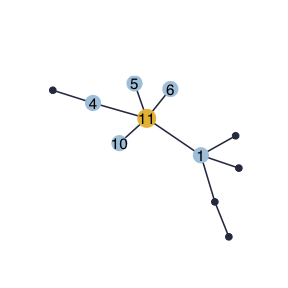
\includegraphics[width=0.3\linewidth]{nestorArticle/man/figures/README-unnamed-chunk-2-1} \end{center}

The original clique of the missing actor neighbors is available in the
value \texttt{TC}:

\begin{Shaded}
\begin{Highlighting}[]
\NormalTok{data}\OperatorTok{\$}\NormalTok{TC}
\CommentTok{#> [[1]]}
\CommentTok{#> [1]  1  4  5  6 10}
\end{Highlighting}
\end{Shaded}

The data is then prepared for analysis with the first step of the
procedure: fit the PLN model. The \texttt{norm\_PLN()} function is a
wraper to \texttt{PLNmodels::PLN()} which normalizes all the necessary
outputs, namely the mean, variance and correlation matrices of the model
latent Gaussian layer corresponding to observed species.

\begin{Shaded}
\begin{Highlighting}[]
\NormalTok{PLNfit<-}\KeywordTok{norm_PLN}\NormalTok{(data}\OperatorTok{\$}\NormalTok{Y)}
\NormalTok{MO<-PLNfit}\OperatorTok{\$}\NormalTok{MO}
\NormalTok{SO<-PLNfit}\OperatorTok{\$}\NormalTok{SO}
\NormalTok{sigma_obs=PLNfit}\OperatorTok{\$}\NormalTok{sigma_obs}
\end{Highlighting}
\end{Shaded}

\subsection{Inference}\label{inference}

\subsubsection{Single clique
initialization}\label{single-clique-initialization}

\texttt{nestor} then needs to be initialized. This requires to find an
initial clique of neighbors for the missing actor, for example using the
\texttt{FitSparsePCA()} function:

\begin{Shaded}
\begin{Highlighting}[]
\NormalTok{initClique =}\StringTok{ }\KeywordTok{FitSparsePCA}\NormalTok{(data}\OperatorTok{\$}\NormalTok{Y,}\DataTypeTok{r=}\DecValTok{1}\NormalTok{, }\DataTypeTok{min.size =} \DecValTok{3}\NormalTok{)}\OperatorTok{\$}\NormalTok{cliques}
\NormalTok{initClique}
\CommentTok{#> [[1]]}
\CommentTok{#> [1]  2  5  7  9 10}
\end{Highlighting}
\end{Shaded}

The \texttt{min.size} parameter defines the minimal size of the output
clique. The function \texttt{init\_mclust()} is also available for
finding a clique, it uses the package \texttt{mclust}.

Once an initial clique has been found, the algorithm can be initialized.
This is the aim of the function \texttt{initVEM()}, which initializes
all required parameters. This function builds one initialization from
one initial clique. We initialize with the clique previously identified:

\begin{Shaded}
\begin{Highlighting}[]
\NormalTok{initList =}\StringTok{ }\KeywordTok{initVEM}\NormalTok{(data}\OperatorTok{\$}\NormalTok{Y, }\DataTypeTok{cliqueList=}\NormalTok{initClique, sigma_obs, MO, }\DataTypeTok{r=}\DecValTok{1}\NormalTok{ )}
\end{Highlighting}
\end{Shaded}

Then to set the tempering parameter \texttt{alpha}, we can look at the
output of the \texttt{alphaMax()} function.

\begin{Shaded}
\begin{Highlighting}[]
\KeywordTok{alphaMax}\NormalTok{(p}\OperatorTok{+}\NormalTok{r, n)}
\CommentTok{#> [1] 0.3000768}
\end{Highlighting}
\end{Shaded}

The actual tempering parameter should be lower than the upper bound
given by \texttt{alphaMax()}. Here we set \texttt{alpha} to \(0.1\). The
core function \texttt{nestor()} can now be run as follows:

\begin{Shaded}
\begin{Highlighting}[]
\NormalTok{fit =}\StringTok{ }\KeywordTok{nestor}\NormalTok{(data}\OperatorTok{\$}\NormalTok{Y, MO,SO, }\DataTypeTok{initList=}\NormalTok{initList, }\DataTypeTok{alpha=}\FloatTok{0.1}\NormalTok{, }\DataTypeTok{eps=}\FloatTok{1e-3}\NormalTok{, }
           \DataTypeTok{maxIter=}\DecValTok{30}\NormalTok{)}
\CommentTok{#> }
\CommentTok{#> nestor ran in 1.078secs and 24 iterations.}
\end{Highlighting}
\end{Shaded}

The object \texttt{fit} contains inferred means and variances of the
complete data, as well as edges weight and probability matrices.

This package contains several visualization functions.
\texttt{plotPerf()} gives a quick overview of the fit performance
compared to initial graph:

\begin{Shaded}
\begin{Highlighting}[]
\KeywordTok{plotPerf}\NormalTok{(fit}\OperatorTok{\$}\NormalTok{Pg, data}\OperatorTok{\$}\NormalTok{G,}\DataTypeTok{r=}\DecValTok{1}\NormalTok{)}
\end{Highlighting}
\end{Shaded}

\begin{center}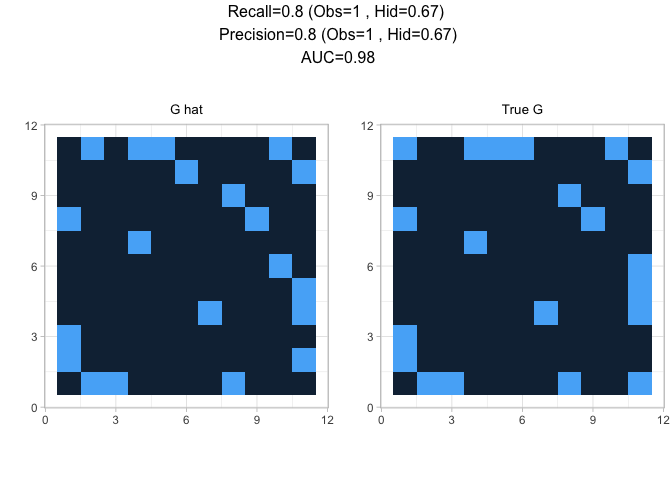
\includegraphics[width=0.8\linewidth]{nestorArticle/man/figures/README-unnamed-chunk-9-1} \end{center}

The convergence of \texttt{nestor()} can be checked with the plotting
function \texttt{plotConv()}:

\begin{Shaded}
\begin{Highlighting}[]
\KeywordTok{plotConv}\NormalTok{(}\DataTypeTok{nestorFit =}\NormalTok{ fit)}
\end{Highlighting}
\end{Shaded}

\begin{center}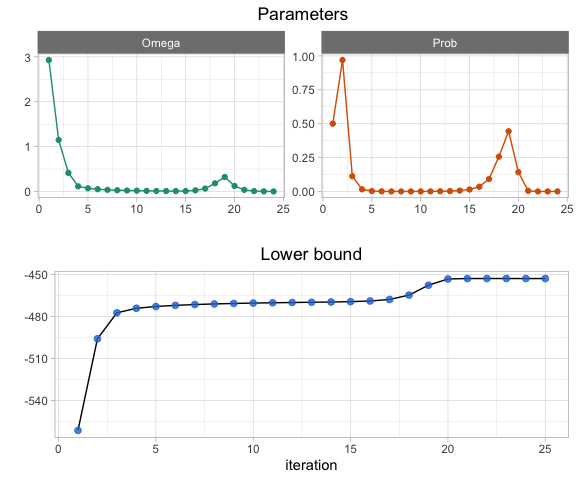
\includegraphics[width=0.8\linewidth]{nestorArticle/man/figures/README-unnamed-chunk-10-1} \end{center}

\subsubsection{Initialization with a list of
cliques}\label{initialization-with-a-list-of-cliques}

The fit of the \texttt{nestor()} function is very sensitive to the
initialization, and so it is recommanded to try several initial cliques.
Several functions are available for finding a list of possible starting
points:

\begin{itemize}
\tightlist
\item
  \texttt{init\_blockmodels()} uses package \texttt{blockmodels},
\item
  \texttt{boot\_FitSparsePCA()} is a bootstraped version using
  \texttt{sparsepca},
\item
  \texttt{complement\_spca()} looks in the complement of the
  \texttt{sparsepca} output.
\end{itemize}

Here we use the \texttt{complement\_spca()} function, which runs
\texttt{sparsepca} and returns the cliques corresponding to the
\texttt{k} first principal components as well as their complement.

\begin{Shaded}
\begin{Highlighting}[]
\NormalTok{six_cliques =}\StringTok{ }\KeywordTok{complement_spca}\NormalTok{(data}\OperatorTok{\$}\NormalTok{Y, }\DataTypeTok{k=}\DecValTok{3}\NormalTok{) }
\NormalTok{six_cliques}
\CommentTok{#> [[1]]}
\CommentTok{#> [[1]][[1]]}
\CommentTok{#> [1] 2 9}
\CommentTok{#> }
\CommentTok{#> [[2]]}
\CommentTok{#> [[2]][[1]]}
\CommentTok{#> [1]  7 10}
\CommentTok{#> }
\CommentTok{#> [[3]]}
\CommentTok{#> [[3]][[1]]}
\CommentTok{#> [1]  2  5 10}
\CommentTok{#> }
\CommentTok{#> [[4]]}
\CommentTok{#> [[4]][[1]]}
\CommentTok{#> [1]  1  3  4  5  6  7  8 10}
\CommentTok{#> }
\CommentTok{#> [[5]]}
\CommentTok{#> [[5]][[1]]}
\CommentTok{#> [1] 1 2 3 4 5 6 8 9}
\CommentTok{#> }
\CommentTok{#> [[6]]}
\CommentTok{#> [[6]][[1]]}
\CommentTok{#> [1] 1 3 4 6 7 8 9}
\end{Highlighting}
\end{Shaded}

This package provides with a parllel procedure for the computation of
several fits of \texttt{nestor()} corresponding to a list of possible
cliques, with the function \texttt{List.nestor()}. Below is an example
with the list of six cliques previously obtained with the
\texttt{complement\_spca()} function:

\begin{Shaded}
\begin{Highlighting}[]
\NormalTok{fitList=}\KeywordTok{List.nestor}\NormalTok{(six_cliques, data}\OperatorTok{\$}\NormalTok{Y, sigma_obs, MO,SO,}\DataTypeTok{r=}\DecValTok{1}\NormalTok{,}
\DataTypeTok{eps=}\FloatTok{1e-3}\NormalTok{,} \DataTypeTok{maxIter =} \DecValTok{50}\NormalTok{, }\DataTypeTok{alpha=}\FloatTok{0.1}\NormalTok{)}
\end{Highlighting}
\end{Shaded}

The object \texttt{fitList} is simply the list of all the
\texttt{nestor()} fits. This procedure aborts in case of degenerated
behaviour, which happens when the provided clique is too far from truth.
Wrong fits can be identified by their ouput size:

\begin{Shaded}
\begin{Highlighting}[]
\KeywordTok{do.call}\NormalTok{(rbind,}\KeywordTok{lapply}\NormalTok{(fitList, length))}
\CommentTok{#>      [,1]}
\CommentTok{#> [1,]    3}
\CommentTok{#> [2,]   12}
\CommentTok{#> [3,]    3}
\CommentTok{#> [4,]   12}
\CommentTok{#> [5,]   12}
\CommentTok{#> [6,]   12}
\end{Highlighting}
\end{Shaded}

Finally we can assess the performance of each converged fit with their
AUC, precision and recall regarding the hidden node \texttt{h}, and the
correlation between the inferred means and the original latent Gaussian
vector of \texttt{h}.

\begin{Shaded}
\begin{Highlighting}[]
\KeywordTok{do.call}\NormalTok{(rbind,}\KeywordTok{lapply}\NormalTok{(fitList, }\ControlFlowTok{function}\NormalTok{(vem)\{}
  \ControlFlowTok{if}\NormalTok{(}\KeywordTok{length}\NormalTok{(vem)}\OperatorTok{>}\DecValTok{4}\NormalTok{)\{}
\NormalTok{    perf=}\KeywordTok{ppvtpr}\NormalTok{(vem}\OperatorTok{\$}\NormalTok{Pg, data}\OperatorTok{\$}\NormalTok{G, }\DataTypeTok{r=}\NormalTok{r)}
    \KeywordTok{c}\NormalTok{(}\DataTypeTok{auc=}\KeywordTok{auc}\NormalTok{(vem}\OperatorTok{\$}\NormalTok{Pg, data}\OperatorTok{\$}\NormalTok{G),}\DataTypeTok{precH=}\NormalTok{perf}\OperatorTok{\$}\NormalTok{PPVH, }\DataTypeTok{recH=}\NormalTok{perf}\OperatorTok{\$}\NormalTok{TPRH, }
    \DataTypeTok{corMH=}\KeywordTok{cor}\NormalTok{(vem}\OperatorTok{\$}\NormalTok{M[,p}\OperatorTok{+}\NormalTok{r], data}\OperatorTok{\$}\NormalTok{UH))}
\NormalTok{  \}}
\NormalTok{\})) }\OperatorTok\StringTok{ }\KeywordTok{as_tibble}\NormalTok{()  }
\CommentTok{#> # A tibble: 4 x 4}
\CommentTok{#>     auc precH  recH  corMH}
\CommentTok{#>   <dbl> <dbl> <dbl>  <dbl>}
\CommentTok{#> 1  0.81  0.6   0.5  -0.785}
\CommentTok{#> 2  0.93  0.75  1    -0.815}
\CommentTok{#> 3  0.76  0.5   0.67 -0.715}
\CommentTok{#> 4  0.69  0.43  0.5  -0.585}
\end{Highlighting}
\end{Shaded}


 